% Source-coordinate reconstruction. Edit named defaults or copy this entire composition.
\studiodeclarefield{graphic-1}{
\includegraphics[width=460\studiounit]{images/studio/collection/figma-0084-part-01.pdf}}
\studiodeclarefield{graphic-2}{
\includegraphics[width=460\studiounit]{images/studio/collection/figma-0084-part-02.pdf}}
\studiodeclarefield{graphic-3}{
\includegraphics[width=460\studiounit]{images/studio/collection/figma-0084-part-03.pdf}}
\studiodeclarefield{graphic-4}{
\includegraphics[width=460\studiounit]{images/studio/collection/figma-0084-part-04.pdf}}
\studiodeclarefield{graphic-5}{
\includegraphics[width=460\studiounit]{images/studio/collection/figma-0084-part-05.pdf}}
\studiodeclarefield{graphic-6}{
\includegraphics[width=580\studiounit]{images/studio/collection/figma-0084-part-06.pdf}}
\studiodeclarefield{graphic-7}{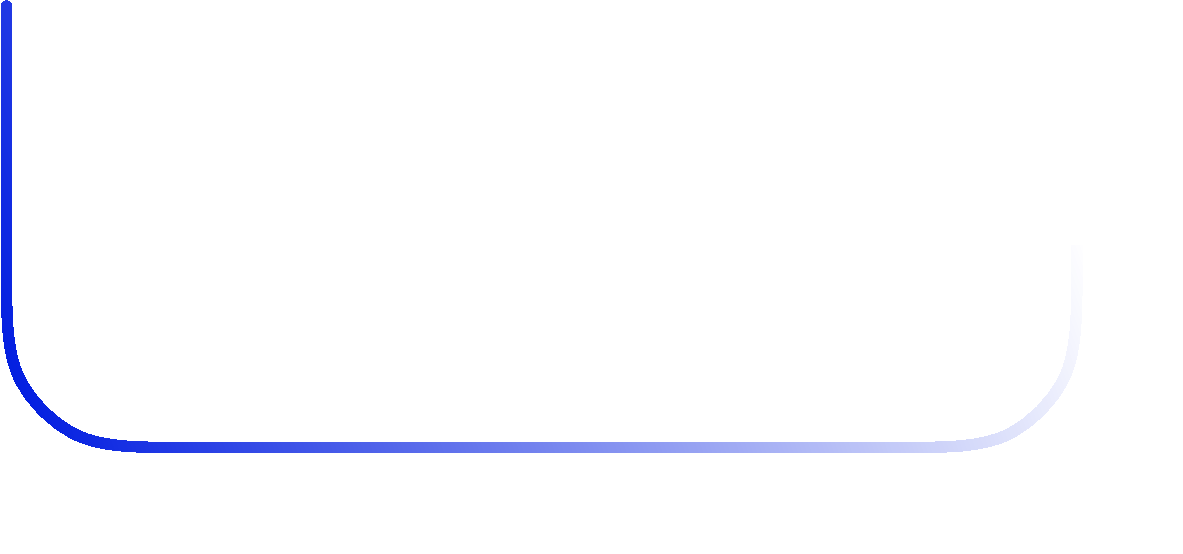
\includegraphics[width=568\studiounit]{images/studio/collection/figma-0084-part-07.pdf}}
\studiodeclarefield{graphic-8}{
\includegraphics[width=568\studiounit]{images/studio/collection/figma-0084-part-08.pdf}}
\studiodeclarefield{graphic-9}{
\includegraphics[width=568\studiounit]{images/studio/collection/figma-0084-part-09.pdf}}
\studiodeclarefield{graphic-10}{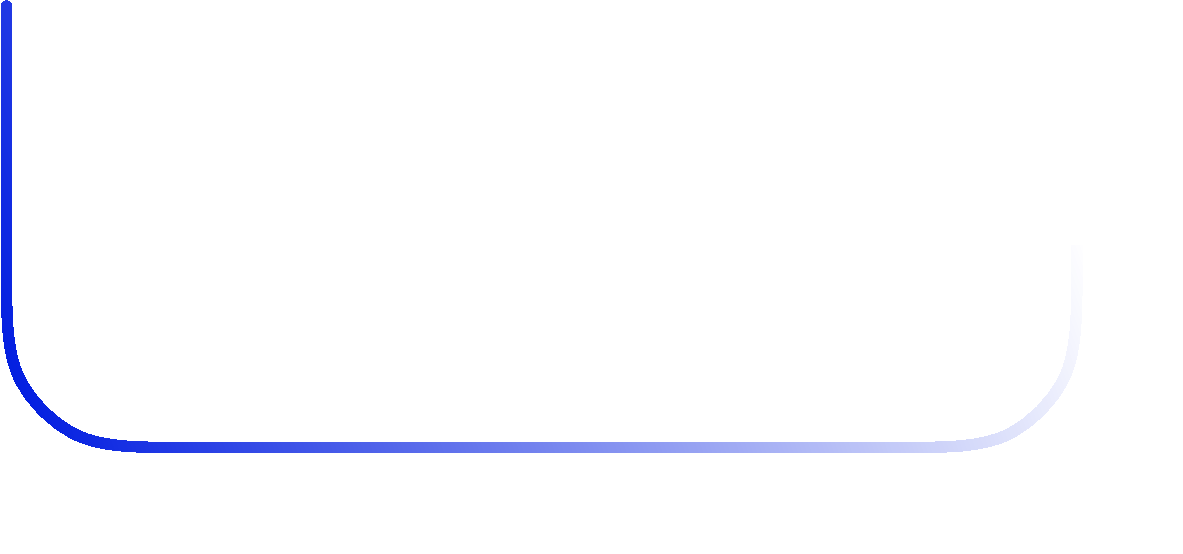
\includegraphics[width=568\studiounit]{images/studio/collection/figma-0084-part-10.pdf}}
\studiodeclarefield{title}{The DAO hack}
\studiodeclarefield{text-2}{Ethereum idea\\proposed by\\Vitalik Buterin}
\studiodeclarefield{text-3}{2014}
\studiodeclarefield{text-4}{July 2015}
\studiodeclarefield{text-5}{April 2016}
\studiodeclarefield{text-6}{June 2016}
\studiodeclarefield{text-7}{June 2016}
\studiodeclarefield{text-8}{The DAO kicks\\off and starts\\fundraising}
\studiodeclarefield{text-9}{Hard fork results\\in Ethereum and\\Ethereum Classic}
\studiodeclarefield{text-10}{Ethereum is\\launched}
\studiodeclarefield{text-11}{The DAO is\\hacked}
\studioapplyfields
\studiomeasuredcanvas{3556}{2000}{horizontal-timeline}{studio-paper}{
\studiomeasuredtext{title}{1366.17}{227.984}{827.739}{149.484}{112.735}{130.772}{\color{bitpolito}\bfseries\centering}{\studiofield{title}}
\studiomeasuredtext{text-2}{532.699}{776.711}{371.64}{200.27}{51.6693}{59.9364}{\color{bitpolito}}{\studiofield{text-2}}
\studiomeasuredtext{text-3}{540.867}{670.742}{132.361}{56.866}{43.74}{50.7384}{\color{bitpolito}\bfseries}{\studiofield{text-3}}
\studiomeasuredtext{text-4}{1053.68}{1300.74}{227.537}{64.0837}{43.7467}{50.7461}{\color{bitpolito}\bfseries}{\studiofield{text-4}}
\studiomeasuredtext{text-5}{1578.62}{666.734}{237.958}{65.014}{43.74}{50.7384}{\color{bitpolito}\bfseries}{\studiofield{text-5}}
\studiomeasuredtext{text-6}{2079.68}{1300.74}{243.876}{56.8727}{43.7467}{50.7461}{\color{bitpolito}\bfseries}{\studiofield{text-6}}
\studiomeasuredtext{text-7}{2599.68}{667.742}{243.872}{56.866}{43.74}{50.7384}{\color{bitpolito}\bfseries}{\studiofield{text-7}}
\studiomeasuredtext{text-8}{1573.67}{773.602}{379.652}{210.195}{52.4213}{60.8087}{\color{bitpolito}}{\studiofield{text-8}}
\studiomeasuredtext{text-9}{2601.63}{773.684}{442.757}{200.379}{51.6693}{59.9364}{\color{bitpolito}}{\studiofield{text-9}}
\studiomeasuredtext{text-10}{1056.09}{1116.71}{308.044}{134.265}{51.6667}{59.9333}{\color{bitpolito}}{\studiofield{text-10}}
\studiomeasuredtext{text-11}{2080.32}{1116.6}{295.85}{134.784}{52.4133}{60.7995}{\color{bitpolito}}{\studiofield{text-11}}
\path[fill=bitpolito,draw=none,line width=1\studiounit] (488.5,1002.5) circle[radius=32.5\studiounit];
\path[fill=bitpolito,draw=none,line width=1\studiounit] (3068.5,1002.5) circle[radius=32.5\studiounit];
\studiographfield{graphic-1}{552}{994}{460}{64}{}{}
\studiographfield{graphic-2}{1065}{994}{460}{64}{}{}
\studiographfield{graphic-3}{1578}{994}{460}{64}{}{}
\studiographfield{graphic-4}{2091}{994}{460}{64}{}{}
\studiographfield{graphic-5}{2604}{994}{460}{64}{}{}
\studiographfield{graphic-6}{485}{739}{580}{266}{}{}
\studiographfield{graphic-7}{1012}{1047}{568}{266}{}{}
\studiographfield{graphic-8}{1526}{736}{568}{266}{}{}
\studiographfield{graphic-9}{2552}{736}{568}{266}{}{}
\studiographfield{graphic-10}{2038}{1047}{568}{266}{}{}
\path[fill=bitpolito,draw=none,line width=1\studiounit] (1014.5,1002.5) circle[radius=19.5\studiounit];
\path[fill=bitpolito,draw=none,line width=1\studiounit] (1527.5,1002.5) circle[radius=19.5\studiounit];
\path[fill=bitpolito,draw=none,line width=1\studiounit] (2040.5,1002.5) circle[radius=19.5\studiounit];
\path[fill=bitpolito,draw=none,line width=1\studiounit] (2553.5,1002.5) circle[radius=19.5\studiounit];
}
